\documentclass[12pt,oneside,a4paper]{article} % for sharing
\usepackage{apacite}
\usepackage{appendix}
\usepackage{amsmath}
\usepackage{amsthm}

\usepackage{amssymb} % for approx greater than
\usepackage{caption}
\usepackage{placeins} % for \FloatBarrier
\usepackage{graphicx}
\usepackage{subcaption}
\usepackage{longtable}
\usepackage{setspace}
\usepackage{booktabs}
\usepackage{tabularx}
\usepackage{xcolor,colortbl}
\usepackage{chngpage}
\usepackage{natbib}
\bibpunct{(}{)}{,}{a}{}{;} 
\usepackage{url}
\usepackage{nth}
\usepackage{authblk}
\usepackage[most]{tcolorbox}
\usepackage[normalem]{ulem}
\usepackage{amsfonts}
% columns for longtable
\usepackage{arydshln} % Dashed lines in matrices

\usepackage[margin=1in]{geometry}
%\doublespacing % for review

% line numbers to make review easier
%\usepackage{lineno}
%\linenumbers

%\usepackage{soul}% for \st{}

%%%%%%%%%%%%%%%%%%%%%%%%%%%%%%%%%%%%%%%%%%%%%%%%%%%%%%%%%%%%%%%%%%%%%%%%%%%%%%
% for section 4 math environments
\theoremstyle{definition}
\newtheorem{definition}{Definition}[section]
\newtheorem{theorem}{Theorem}[section]
\newtheorem{proposition}{Proposition}[section]
\newtheorem{corollary}{Corollary}[proposition]
\newtheorem{remark}{Remark}[section]

%%%%%%%%%%%%%%%%%%%%%%%%%%%%%%%%%%%%%%%%%%%%%%%%%%%%%%%%%%%%%%%%%%%%%%%%%%%%%%

\newcommand\ackn[1]{%
  \begingroup
  \renewcommand\thefootnote{}\footnote{#1}%
  \addtocounter{footnote}{-1}%
  \endgroup
}

% Affiliations in small font size
\renewcommand\Affilfont{\small}

\defcitealias{HMD}{HMD 2016}

% junk for longtable caption
\AtBeginEnvironment{longtable}{\linespread{1}\selectfont}
\setlength{\LTcapwidth}{\linewidth}

% sort van Raalte properly
% #1: sorting key, #2: prefix for citation, #3: prefix for bibliography
\DeclareRobustCommand{\VAN}[3]{#2} % set up for citation
\newcommand{\tc}{\quad\quad\text{,}}
\newcommand{\tp}{\quad\quad\text{.}}
%%%%%%%%%%%%%%%%%%%%%%%%%%%%%%%
\begin{document}

\title{Symmetry in the forward and backward tenure of transient states in
stationary populations}
%\author{author(s) redacted}
\author[1]{Tim Riffe\thanks{riffe@demogr.mpg.de}}
\author[2,3]{Francisco Villavicencio}
\affil[1]{Max Planck Institute for Demographic Research, Rostock, Germany}
\affil[2]{Max-Planck Odense Center on the Biodemography of Aging, Odense, Denmark}
\affil[3]{Department of Public Health, University of Southern Denmark, Odense, Denmark}

\maketitle

\begin{abstract}

\end{abstract}

A perfectly stationary population is either perfectly stationary because it is
of infinite size or because it is finite and deterministically repeating.
Assuming that individuals in a stationary population can obtain different states
through life, we take for granted that the age-state structure is also invariant
over time. The population may indeed be heterogenous in the sense that different
states may have different vital rates. However, everything is fixed in such a
way that birth cohorts are of fixed size, and the numbers of people in each age
and state are the same in each time step. Further, the distribution of
state-specific tenures for individuals entering a state at a given age is also a
fixed attribute, by consequence of the former requisites of stationarity. 

It is by now well-established via the Brouard-Carey equality
\citep{brouard1989mouvements,Vaupel2009,rao2014,villavicencioRiffeSymmetires2016}
that the distributions of years-lived and years-left are identical in perfectly stationary populations.



\section{An intuitive proof of transient symmetry}

\begin{theorem}
Given a continuous (or infinite) stationary population and fixed transition
rates, the probability that a randomly selected individual is in state $s$ and entered the state $x$ years
ago is equal to the probability of being in state $s$ and exiting in $x$ years.
\end{theorem}

\begin{proof}
The proof of this statement unfolds in five intuitive steps.
\begin{enumerate}
\item{} A duration can be represented as a line segment, potentially a
subset of a life-line. Points along a single within-person duration could be continuously
sampled over time, used to bisect the segment, collecting two infinite sets of
values: time spent in the duration and time until exiting the duration. If
continuously collected, these two sets will have the same values, with time
spent in ascending order and time left in descending order. If sorted
identically these two sets will therefore be identical. This is so by way of
complements.

If the duration in question is called $d^i$, the date of entry is $d_L^i$ and
the date of exit is $d_R^i$, then the length of $d^i$ is $d_R^i - d_L^i$ and the
set of time spent values, $A^i$ is defined as:
\begin{align}
\label{eq:Ai}
A^i &= \{a \in \mathbb{R}~ | ~0 \le a \le (d_R^1 - d_L^1) \} \tc
\intertext{and the
set of time left values, $T^1$ is also:}
\label{eq:Ti}
T^i &= \{a \in \mathbb{R}~ | ~ (d_R^1 - d_L^1) \ge a \ge 0 \} \tc
\end{align}

Figure~\ref{fig:lifeline1} illustrates the construction of $A^i$ and $T^i$ in
expressions~\eqref{eq:Ai} and \eqref{eq:Ti}. The central cutpoint moves along
the duration from the time of entry until the time of exit, creating two
infinite sets.

\begin{figure}
\centering
\caption{A lifeline of individual $i$ showing the construction of the sets $A^i$
and $T^i$.}
\label{fig:lifeline1}
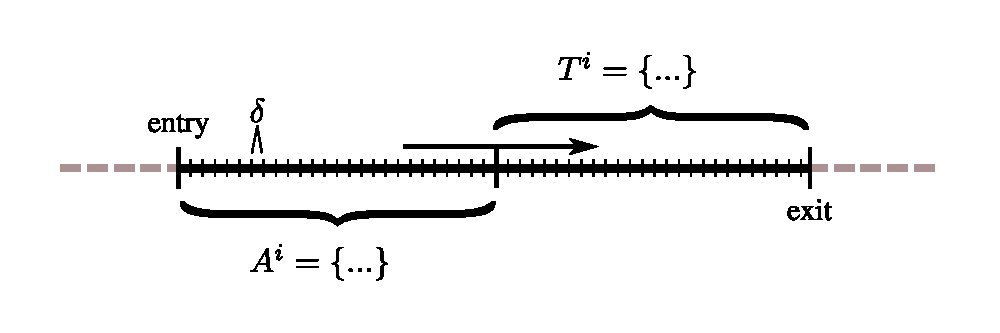
\includegraphics[scale=.8]{Figures/lifeline1.pdf}
\end{figure}

\FloatBarrier
\item{} If this individual is reborn in each instant, destined to relive the
exact same life course as the first, we end up with an infinite
number of identically aligned and identically long segments placed side-by-side.
This infinite set of segments in effect forms a plane. One could in this
setting take a census at a single point in time, collecting an infinite set of
time spent and time left values, each from a unique cohort in sequence. It is
clear that the two sets observed at a single time point will be identical
to the first two sets that were observed of a single duration over its entire
length.

Figure~\ref{fig:clones} illustrates this notion with finely-spaced lifelines in
a Lexis configuration, which the reader can imagine forming a continuos
plane. The vertical line indicates a hypothetical census at time $t$ of
the continuously-aged population of this clones individual. At time $t$, the blue-highlighted segments indicate
the set of time-spent values in $A^i$, and red-highlighted segments are the
time-left elements of $T^i$. 

 \begin{figure}[h!]
\centering
\caption{The life of individual $i$ repeated continuosly over time. A
census with followup now constructs the sets $A^i$ and $T^i$ with values
identical to the within-individual sets.}
\label{fig:clones}
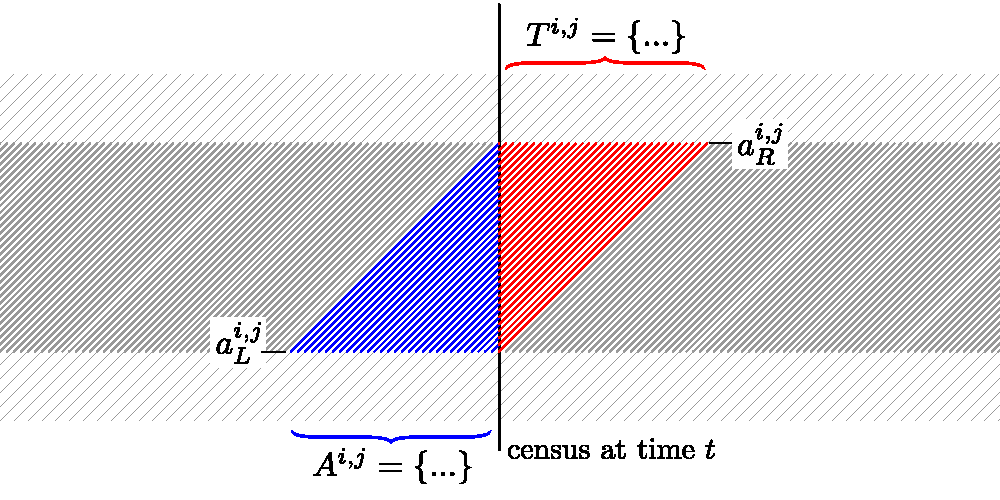
\includegraphics[scale=.8]{Figures/lifelinerepeated.pdf}
\end{figure}

Formally, sets $A^i$ and $T^i$ consist of the same values as the previous, but
coming from individuals born in a continuous flow from $d_R^1 - t$ years ago
until as recently as $d_L^1 - t$ years ago. This is a sort of demonstration of
both period-cohort equality, but also of time spent-left equality. The blue
and red triangles in Figure~\ref{fig:clones} are simple rotations of one
another.

\FloatBarrier
\item{} Assume we have a second individual from the same birth cohort that
enters the same state as the first, but at a different time and for a different total
duration. We could demonstrate time spent and time left equality in the same
way for this individual, by sampling continously over time. Since this
individual has a different lifecourse timing than the first individual, their sets of time-spent, $A^2$, and time left $T^2$
will be distinct. $A^1$ and $T^1$ range from 0 to $d^1$, whereas $A^2$ and $T^2$
range from 0 to $d^2$. However, their unions are identical:

\begin{equation}
\label{eq:unioneq}
\{A^1 \cup A^2\} = \{T^1 \cup T^2\}
\end{equation}

\item{} If the second individual is perfectly clones continously over time as in
step 2, then our census at a single point in time also yields
identical sets of time spent and time left values. Also from this census, the union of the
first and second time-spent sets and the union of the first and second time-left sets
are guaranteed to be identical, as in equation \eqref{eq:unioneq}. 

\item{} By induction we can keep adding durations in this state, infinitely if we
please, and the union of all resultant time-spent sets and the union of time-left sets will continue being identical. Therefore the
probability of selecting a particular value from the time-spent set is identical
to the probability of selecting the same value from the time-left set. This
constitutes a proof of symmetry of time spent and left in transient states in
stationary populations.
\end{enumerate}
\end{proof}

\section{Discussion}
This approach from this proof is equally valid to proove the
original statement of the Brouard-Carey equality, but it is more general. The
statement and proof is so flexible as to hold for irreversible and reversible
states. It is also applicable to repeatible states, whether time spent in the
state is kept in cumulative fashion over spells, or whether the clock resets to
zero on each entry into the state. The equality may also be conditionable in
curious ways: for example, the distribution of time-spent in a state conditional
on having entered at age $a$ must also be equal to the distribution of time-left in
the state, $a$.

Prior to proof, this equality is probably less intuitive than the Brouard-Carey
equality, because state entry is not necessarily aligned on each zero. It is
therefore less visible in commonly-produced plots. It might be tempting to think
that due to state-varying vital rates, that the equality simply ought not hold.
However, the basis of the proof is the observation that if each individual
duration is symmetrical by complements, then so are aggregations of
durations, irrespective of alignment. 

Empirical applications of the presently-described transient tenure equality may
be easy to conjure up. For example, imagine a hypothetical health state that
shows no consequential or noticeable symptoms, but is medically measureable. One
may take a census with regular follow-ups, until eventually the state is exited
by each individual, whether by absorbtion into death or entry into another
state. Then, if the assumption of stationarity is acceptible, one may be able to
say something about onset timing in the aggregate, itself unobserved. We think
that the present equality will come as good news to researchers in similar
settings.

\bibliographystyle{chicago}
\bibliography{references}  
\end{document}
